\documentclass[11pt,a4paper,parskip=half]{scrartcl}
\usepackage{ngerman}
\usepackage[utf8]{inputenc}
\usepackage[colorlinks=false,pdfborder={0 0 0}]{hyperref}
\usepackage{graphicx}
\usepackage{caption}
\usepackage{longtable}
\usepackage{float}
\usepackage{textcomp}
\usepackage{geometry}
\usepackage{amsmath}
\usepackage{amssymb}
\geometry{a4paper, left=30mm, right=25mm, top=30mm, bottom=35mm} 
\usepackage{listings}
\lstset{breaklines=true, breakatwhitespace=true, basicstyle=\scriptsize, numbers=left}
\title{Workshop System Management}
\author{Tobias Lerch, Yanick Eberle, Pascal Schwarz}
\begin{document}
\maketitle
\newpage

\tableofcontents
\newpage

\section{Netzwerk}
\subsection{Netzwerkdiagramm}
\begin{figure}[H]
\centering
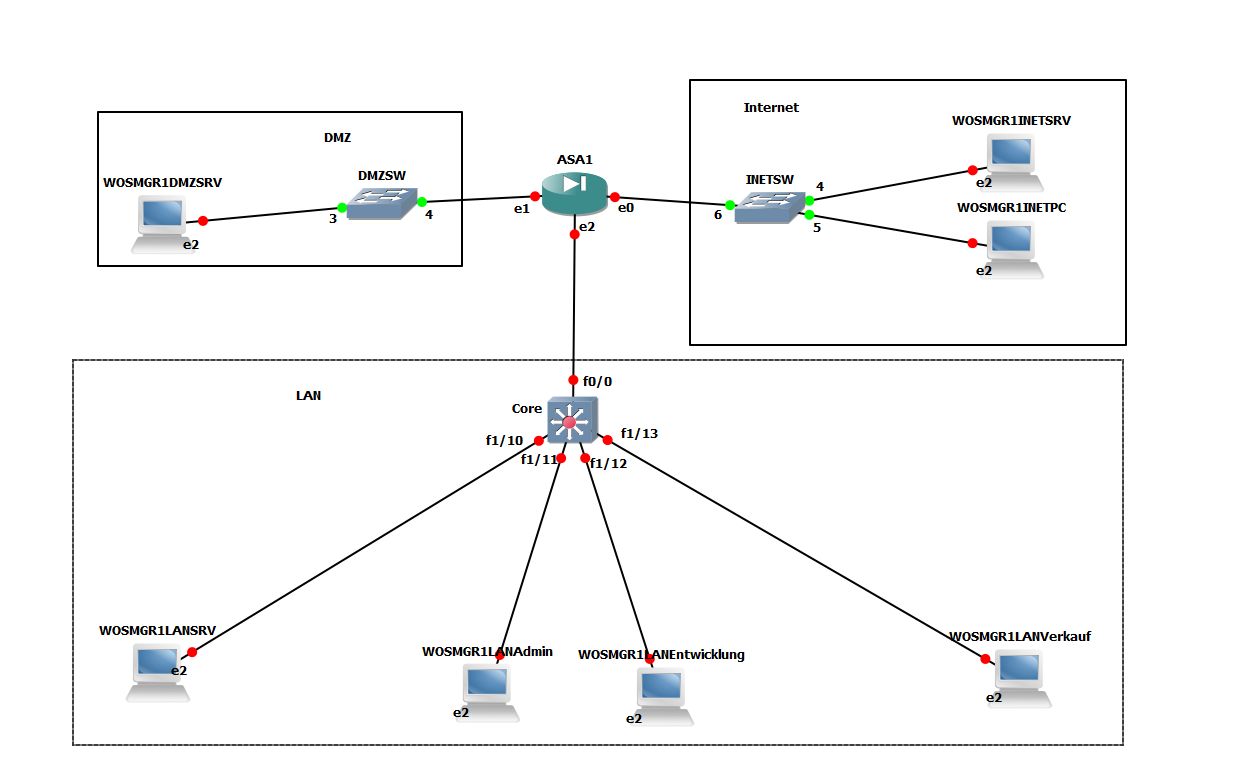
\includegraphics[width=1.0\textwidth]{Phase1/Netz.PNG}
\caption{Netzwerk}
\label{fig:netzwerkdiagramm}
\end{figure}

\subsection{IP Dual-Stack Konzept}
\subsubsection{IPv4}
Wir unterscheiden zwischen drei verschiedenen Netzwerke. Das interne Netzwerk, das DMZ Netzwerk und das öffentliche Netzwerk. Wir verwenden für die DMZ und das interne Netzwerk verschiedene Netzwerkklassen um die Netze schnell unterscheiden zu können. Folgende IP-Adressierung und Maskierung werden wir verwenden.

\begin{longtable}{p{1.5cm}|p{4cm}|p{4cm}|p{3cm}}
	\textbf{VLAN} & \textbf{Funktion} & \textbf{IPv4 Range} & \textbf{IPv4 Gateway}\\
	\hline
	\endfirsthead
	\textbf{VLAN} & \textbf{Funktion} & \textbf{IPv4 Range} & \textbf{IPv4 Gateway}\\
	\hline
	\endhead
	\hline
	\multicolumn{2}{l}{\textit{Fortführung auf nächster Seite\ldots}} \\
	\endfoot
	\endlastfoot
	10 & Server & 10.0.10.0/24 & 10.0.10.1\\
	20 & Administratoren & 10.0.20.0/24 & 10.0.20.1\\
	30 & Entwicklung & 10.0.30.0/24 & 10.0.30.1\\
	40 & Verkauf & 10.0.40.0/24 & 10.0.40.1\\
	n/a & VPN Clients & 10.0.99.0/24 & n/a \\
	n/a & Infrastructure & 10.100.0.0/30 & n/a\\
	n/a & DMZ & 172.16.0.0/24 & 172.16.0.1\\
	n/a & WAN & 209.165.50.0/24 & 209.165.50.1
\end{longtable}

\subsubsection{IPv6}
Da die Hosts über das Internet direkt erreichbar sein sollen, werden wir globale IPv6 Adressen mit dem Site Prefix /64 verwenden.

\begin{longtable}{p{1.5cm}|p{4cm}|p{4cm}|p{4cm}}
	\textbf{VLAN} & \textbf{Funktion} & \textbf{IPv6 Range} & \textbf{IPv6 Gateway}\\
	\hline
	\endfirsthead
	\textbf{VLAN} & \textbf{Funktion} & \textbf{IPv6 Range} & \textbf{IPv6 Gateway}\\
	\hline
	\endhead
	\hline
	\multicolumn{2}{l}{\textit{Fortführung auf nächster Seite\ldots}} \\
	\endfoot
	\endlastfoot
	10 & Server & 2005:2013:FF:A10::/64 & 2005:2013:FF:A10::1\\
	20 & Administratoren & 2005:2013:FF:A20::/64 & 2005:2013:FF:A20::1\\
	30 & Entwicklung & 2005:2013:FF:A30::/64 & 2005:2013:FF:A30::1\\
	40 & Verkauf & 2005:2013:FF:A40::/64 & 2005:2013:FF:A40::1\\
	n/a & Infrastructure & 2005:2013:FF:A0::/64 & n/a\\
	n/a & DMZ & 2005:2013:FF:B0::/64 & 2005:2013:FF:B0::1/64\\
	n/a & WAN & 2005:209:165:50::/64 & 2005:209:165:50::1/64
\end{longtable}

\subsection{Adressvergabe an Clients}
\subsubsection{IPv4}
Die Clients stellen regulare DHCP-Anfragen. Um die Leases und Bereichsoptionen zentral und (einigermassen) angenehm über eine grafische Schnittstelle verwalten zu können, wird der Core-Router so konfiguriert, dass er die Anfragen an den internen Domänencontroller und DHCP-Server (INTSRV in VLAN10) weiterleitet. Der Router setzt dabei ein Flag in der Anfrage, welches es dem DHCP-Server erlaubt, festzustellen aus welchem Bereich die Anfrage kam. Nur so kann der Server beispielsweise einem Client aus dem Adminnetz eine IP aus dem Admin-Bereich zuweisen.

Der folgende Konfigurationsausschnitt zeigt die notwendigen Optionen (IPv6-betreffende Einstellungen entfernt):
\begin{lstlisting}
interface Vlan20
 description *** VLAN Admin ***
 ip address 10.0.20.1 255.255.255.0
 ip access-group ADMIN in
 ip helper-address 10.0.10.21
\end{lstlisting} 

Der Befehl \glqq{}ip helper address\grqq{} gibt an, wohin die DHCP-Anfrage weitergeleitet werden soll.

\subsubsection{IPv6}
Für die automatische Konfiguration der Client-Adressen für IPv6 kommen mehrere Möglichkeiten in Betracht:
\begin{description}
	\item[Autokonfiguration ohne DHCP] IPv6 sieht vor, dass Router Clients direkt das zu verwendende Netzwerkprefix angeben können und Clients sich dann mittels EUI-64 eine Adresse generieren. Da EUI-64 die (weltweit eindeutige) MAC-Adresse miteinbezieht, sind Adresskonflikte ausgeschlossen. Die Clients erfahren über Router-Advertisements, welche Netze sie über welche Router erreichen können.
		Leider ist keine Möglichkeit vorgesehen, den Clients mitzueteilen, welchen DNS-Server sie verwenden sollen. Somit kann dieser Ansatz alleine aktuell das Problem der Adressvergabe nicht abschliessend lösen.
	\item[DHCPv6 stateful] Diese Variante funktioniert sehr ähnlich wie die klassische DHCP Adressvergabe in IPv4-Netzen. Der Client fragt per Multicast (Broadcast-Adressen wurden in IPv6 abgeschafft) nach DHCP-Servern und \glqq{}bestellt\grqq{} sich eine Adresse. Die Angabe von weiteren Optionen, wie eine Liste der DNS-Server ist genau auf die selbe Art und weise möglich, wie dies bereits in IPv4-Netzen der Fall war. Eine Einschränkung ist bei unserer Konfiguration allerdings ins Gewicht gefallen: Der DHCP-Server kann den Clients keinen Default-Gateway angeben, eine entsprechende Option ist derzeit im Protokoll nicht vorgesehen.
	\item[DHCPv6 stateless] Diese Variante vereint die Stärken der beiden zuvor genannten Varianten der Adressvergabe. Die Konfiguration der IPv6-Adresse sowie des Gateways erfolgt per Router-Advertisements zwischen Router und Client. In der Antwort zur Router-Solicitation-Anfrage des Clients gibt der Router dem Client des Weiteren an, dass er weitere Informationen per DHCPv6 erfragen soll. Als Antwort auf die DHCP-Anfrage erhält der Client dann Optionen wie eine DNS-Serverliste oder den Domänennamen. Die Bezeichnung \glqq{}stateless\grqq{} rührt daher, dass der Server keine Informationen (Lease) zu den Clients speichern muss.
\end{description}

Auch dieser Ansatz soll mit einem Auszug der Schnittstellenkonfiguration verdeutlicht werden (IPv4 betreffende Konfigurationen entfernt):
\begin{lstlisting}
interface Vlan20
 description *** VLAN Admin ***
 ipv6 address 2005:2013:FF:A20::1/64
 ipv6 traffic-filter ADMINv6 in
 ipv6 nd other-config-flag
 ipv6 dhcp relay destination 2005:2013:FF:A10::21
\end{lstlisting}

Die Option \glqq{}ipv6 nd other-config-flag\grqq{} gibt an, dass der Router Clients darauf hinweisen soll, dass weitere Informationen über DHCPv6 erhalten werden können. Eine andere Einstellung hier wäre \glqq{}ipv6 nd managed-config-flag\grqq{} - dies würde den Client auffordern, auch seine IP-Adresse per DHCPv6 zu erfragen.

\glqq{}ipv6 dhcp relay destination\grqq{} gibt, analog zu der \glqq{}helper-adress\grqq{} bei IPv4, an, wohin DHCP-Anfragen weitergeleitet werden sollen.

Des Weiteren ist zu beachten, dass eintreffende \glqq{}Router-Solicitation\grqq{}-Anfragen der Clients nicht durch die ACL geblockt werden. Falls dies dennoch der Fall ist, erhält der Client die IPv6-Route erst nach einiger Zeit, da der Router von sich aus periodisch Router-Advertisement verschickt.

\subsection{Routing}
\subsubsection{Core Router}
Der Core Router hat nur default-routen konfiguriert. Sämtlicher Datenverkehr, der nicht in ein lokal angeschlossenes Netz soll, wird an die Firewall gesendet.

\begin{longtable}{p{4.5cm}|p{4cm}}
	\textbf{Zielnetz} & \textbf{Next Hop}\\
	\hline
	\endfirsthead
	\textbf{Zielnetz} & \textbf{Next Hop}\\
	\hline
	\endhead
	\hline
	\multicolumn{2}{l}{\textit{Fortführung auf nächster Seite\ldots}} \\
	\endfoot
	\endlastfoot
	0.0.0.0/0 & 10.100.0.2\\
	::/0 & 2005:2013:FF:A0::2
\end{longtable}

\subsubsection{Firewall}
Die default Route auf der Firewall würde normalerweise auf den Router des Service Providers zeigen. Da wir in der Simulation aber keinen solchen haben, werden keine default Routen konfiguriert. Die Firewall sendet somit nur den Verkehr für das interne Netzwerk an den Core Router.

\begin{longtable}{p{4.5cm}|p{4cm}}
	\textbf{Zielnetz} & \textbf{Next Hop}\\
	\hline
	\endfirsthead
	\textbf{Zielnetz} & \textbf{Next Hop}\\
	\hline
	\endhead
	\hline
	\multicolumn{2}{l}{\textit{Fortführung auf nächster Seite\ldots}} \\
	\endfoot
	\endlastfoot
	10.0.0.0/16 (Supernet) & 10.100.0.1\\
	2005:2013:FF:A10::/64 & 2005:2013:FF:A0::1\\
	2005:2013:FF:A20::/64 & 2005:2013:FF:A0::1\\
	2005:2013:FF:A30::/64 & 2005:2013:FF:A0::1\\
	2005:2013:FF:A40::/64 & 2005:2013:FF:A0::1
\end{longtable}

\subsection{NAT}
Network Address Translation wird für IPv4 verwendet um den internen Clients Zugriff ins Internet zu gewähren und um den Webserver in der DMZ vom Internet aus zugänglich zu machen. Für den Internetzugriff der Clients wird eine Port Address Translation (PAT) konfiguriert, damit nur eine Public IP-Adresse verwendet werden muss. Für den Webserver wird ein statisches NAT mit einer zusätzlichen Public IP-Adresse konfiguriert.

\begin{description}
	\item[Webserver] statisches NAT interne IP: 172.16.0.21 - öffentliche IP: 209.165.50.2
	\item[Interne Hosts] dynamisches NAT overload: interner Range: 10.0.0.0/16 - öffentliche IP 209.165.50.1 (Outside IF IP der Firewall)
\end{description}
Ausgenommen vom NAT ist die Verbindung vom Server Netzwerk (10.0.10.0/24) ins VPN Client Netzwerk (10.0.99.0/24) da sonst keine Verbindung von Remote Client zu Server erstellt werden kann.

\subsection{VTP}
Das VLAN Trunking Protokoll kommt in unserer Simulation nicht zu Einsatz, da GNS3 keine konfigurierbare Switches anbietet. Im Labor werden wir jedoch mit konfigurierbaren Switches arbeiten und VTP einsetzen. Der Core Router wird dabei der VTP Server sein und alle VLAN Informationen an die Switches verteilen.

\subsection{Spanning-Tree}
Spanning-Tree musste in der Simulation nicht berücksichtigt werden. Das Netzwerk ist sehr einfach aufgebaut und die Verbindung zwischen Core Router und Firewall benötigt keinen Spanning-Tree.

\subsection{VPN IPsec Remote Access}
Der Zugriff auf das interne Netzwerk für externe Mitarbeiter erfolgt über den IPsec VPN Client. Beim Zugriff unterscheiden wir zwischen Administratoren und Mitarbeiter. Der Zugriff als Mitarbeiter kann somit stärker eingeschränkt werden als ein Administrator. In der Simulation haben wir keine unterschiedlichen Zugriffsmöglichkeiten, die Firewall wurde aber für diesen Fall konfiguriert. Der Remote Access Zugang erfolgt über die IP 209.165.50.1 (Outside IF Firewall) und unterstützt nur IPv4.\\
\\
\textbf{IKE Phase 1:}
\begin{itemize}
	\item{Authenzifizierung: Pre-shared}
	\item{Verschlüsselung AES 256-bit}
	\item{Hash SHA}
	\item{Schlüsselgenerierung Diffie-Hellman Group 2}
	\item{Gültigkeit Schlüsse 12h}
\end{itemize}

\textbf{IKE Phase 2 (Group-Policy):}
\begin{itemize}
	\item{Interne Gruppen (VPN\_ADMINISTRATOR \& VPN\_USERS\_GROUP)}
	\item{DNS-Server 10.0.10.21}
	\item{ACL 99: permit ip any 10.0.10.0 255.255.255.0 }
	\item{Split-Tunneling: 10.0.10.0/24}
	\item{Tunnel Protokol IKEv1 \& IKEv2}
	\item{Default Domain: wosm.com}
	\item{IP-Adressen Pools: VPN-ADMIN 10.0.99.0/25, VPN-USERS 10.0.99.128/25}
\end{itemize}

\subsection{Serverkonzept}
\begin{longtable}{p{3cm}|p{2.5cm}|p{2.3cm}|p{3.5cm}|p{3cm}}
	\textbf{Name} & \textbf{OS} & \textbf{IPv4} & \textbf{IPv6} & \textbf{Services}\\
	\hline
	\endfirsthead
	\textbf{Name} & \textbf{OS} & \textbf{IPv4} & \textbf{IPv6} & \textbf{Services}\\
	\hline
	\endhead
	\hline
	\multicolumn{2}{l}{\textit{Fortführung auf nächster Seite\ldots}} \\
	\endfoot
	\endlastfoot
	LANSRV & Windows Server 2008 R2 & 10.0.10.21 & 2005:2013:ff:a10::21 & AD, DNS, DHCP, Fileserver\\
	LANAdmin & Windows 7 & 10.0.20.21 & 2005:2013:ff:a20::21 & Client Admin\\
	LANEntwicklung & Windows 7 & 10.0.30.21 & 2005:2013:ff:a30::21 & Client Entwicklung\\
	LANVerkauf & Windows 7 & 10.0.40.21 & 2005:2013:ff:a40::21 & Client Verkauf\\
	DMZSRV & Windows Server 2008 R2	& 172.16.0.21 & 2005:2013:ff:b0::21	& HTTP, HTTPS, FTP\\
	INETSRV	& Windows Server 2008 R2 & 209.165.50.21 & 2005:209:165:50::21 & HTTP, HTTPS, FTP\\
	INETPC & Windows 7 & 209.165.50.22 & 2005:209:165:50::22 & Client Extern\\
\end{longtable}


\section{Sicherheit}
\subsection{Konzept}
Um die Sicherheit unseres Netzes zu gewähtleisten, haben wir uns entschieden, verschiedene Sicherheitsstufen zu definieren. Dabei verfolgen wir eine High Security Strategie. Die höchste Sicherheitsstufe 'Stufe 1' gilt für die normalen User. Die zweite Sicherheitsstufe 'Stufe 2' gilt für die Server. Die dritte Sicherheitsstufe 'Stufe 3' gilt für die Administratoren.

Bei der Sicherheitsstufe Stufe 1 wird nur das nötigste zugelassen und alles andere blockiert. Die User dürfen über Ports 80 und 443 im Internet surfen, sowie FTP Verbindungen über Port 21 und 20 öffnen. Zudem werden eingehende DHCP Anfragen über den Port UDP 68 zugelassen.

Bei der Sicherheitsstufe Stufe 2 wird alles zugelassen, was die Server benötigen. Dabei wird aus den VLANs 20, 30 und 40 alles zugelassen. Aus der DMZ wird nur der Port 389 für LDAP zugelassen.

Bei der Sicherheitsstufe Stufe 3 wird zusätzlich zu den in Stufe 1 zugelassenen Ports noch der Port 22 im internen Netz und in die DMZ zur Verwaltung der Netzwerkgeräte zugelassen. Zudem ist beim Internetzugang für die Administratoren alles offen.

Die definierten Sicherheitsstufen wurden mithilfe verschiedener ACLs umgesetzt. Die definierten Regeln (Auflistung oben nicht abschliessend) der ACL's sind im folgenden Kapitel ersichtlich.

Die ACLs werden möglichst nahe an der Quelle angewendet. Somit sind alle ACLs welche den Zugriff der verschiedenen internen VLANs in irgend ein anderes Netz regeln auf dem Core Switch auf den VLAN-Interfaces in Richtung \emph{in} angewendet. Alle ACLs die den Zugriff in die DMZ, resp. von der DMZ in ein anderes Netz regeln werden auf der ASA angewendet. Alle ACLs die den eingehenden Traffic aus dem Internet regeln sind ebenfalls auf der ASA angewendet.

Mit einer Stateful Firewall sinkt einerseits der Konfigurationsaufwand und gleichzeitig kann eine höhere Sicherheit erreicht werden. Da wir eine High Security Strategie verfolgen, ist die Stateful Variante besser geeignet für unsere Zwecke.

\subsection{Firewall}
\subsubsection{ACL auf Core-Router}
Auf diesem Router sind ACL für alle angeschlossenen VLANs definiert. Die folgende Tabelle liefert einen Überblick, die kompletten ACL sind im Anhang dieser Dokumentation zu finden.
\begin{longtable}{p{2.5cm}|p{3.5cm}|p{7cm}}
	\textbf{Name} & \textbf{Interface/Richtung} & \textbf{Anmerkung}\\
	\hline
	\endfirsthead
	\textbf{Name} & \textbf{Interface/Richtung} & \textbf{Anmerkung}\\
	\hline
	\endhead
	\hline
	\multicolumn{2}{l}{\textit{Fortführung auf nächster Seite\ldots}} \\
	\endfoot
	\endlastfoot
	INTSRV & VLAN 10 / in & Reglementiert IPv4 Traffic, der aus dem Servernetz verschickt werden darf.\\
	INTSRVv6 & VLAN 10 / in & Reglementiert IPv6 Traffic, der aus dem Servernetz verschickt werden darf.\\
	ADMIN & VLAN 20 / in & Reglementiert IPv4 Traffic, der aus dem Adminnetz verschickt werden darf.\\
	ADMINv6 & VLAN 20 / in & Reglementiert IPv6 Traffic, der aus dem Adminnetz verschickt werden darf.\\
	DEV & VLAN 30 / in & Reglementiert IPv4 Traffic, der aus dem Entwicklungsnetz verschickt werden darf.\\
	DEVv6 & VLAN 30 / in & Reglementiert IPv6 Traffic, der aus dem Entwicklungsnetz verschickt werden darf.\\
	VERKAUF & VLAN 40 / in & Reglementiert IPv4 Traffic, der aus dem Verkaufsnetz verschickt werden darf.\\
	VERKAUFv6 & VLAN 40 / in & Reglementiert IPv6 Traffic, der aus dem Verkaufsnetz verschickt werden darf.\\
\end{longtable}

\subsubsection{ACL auf ASA}
Auf der Firewall wurden jeweils 3 Access Lists definiert. Diese werden auf den jeweiligen Interfaces angewendet. Die kompletten Access-lists sind im Anhang zu finden.

\begin{longtable}{p{2.5cm}|p{3.5cm}|p{7cm}}
	\textbf{Name} & \textbf{Interface/Richtung} & \textbf{Anmerkung}\\
	\hline
	\endfirsthead
	\textbf{Name} & \textbf{Interface/Richtung} & \textbf{Anmerkung}\\
	\hline
	\endhead
	\hline
	\multicolumn{2}{l}{\textit{Fortführung auf nächster Seite\ldots}} \\
	\endfoot
	\endlastfoot
	dmz\_in & dmz / in & IPv4 Traffic, der aus dem DMZ-Netzwerk verschickt werden darf.\\
	dmz\_in\_v6 & dmz / in & IPv6 Traffic, der aus dem DMZ-Netzwerk verschickt werden darf.\\
	inside\_in  & inside / in & IPv4 Traffic, der aus dem internen Netzwerk verschickt werden darf.\\
	inside\_in\_v6 & inside / in & IPv6 Traffic, der aus dem internen Netzwerk verschickt werden darf.\\
	outside\_in & outside / in & IPv4 Traffic, der aus dem Internet verschickt werden darf.\\
	outside\_in\_v6 & outside / in & IPv6 Traffic, der aus dem Internet verschickt werden darf.\\
\end{longtable}

\section{Bedrohungsmodell}
\subsection{TCP DoS (SYN-Flooding)}
\subsubsection{Bedrohung}
Beim TCP 3-Way Handshake wird zuerst eine Anfrage an einen Server gesendet, indem ein TCP Paket mit dem Flag SYN verschickt wird. Der Server als Empfänger dieses TCP SYN Pakets verarbeitet dieses und sendet ein TCP Paket mit den Falgs SYN und ACK zurück. Er merkt sich dabei in einer SYN-Liste, mit wem er ein 3-Way Handshake begonnen hat. Wenn derInitiator der Verbindung das TCP Paket mit den Flags SYN und ACK empfängt, verarbeitet er dieses und sendet zur Bestätigung ein Paket mit dem Flag ACK. Sobald der Server das Packet mit dem Flag ACK erhalten hat, wird der Eintrag in der SYN-Liste gelöscht.\\
Ein Angreifer sendet 100 SYN-Anfragen pro Sekunde an einen bestimmten Server. Dabei setzt er eine andere Source IP Adresse, sodass die Antwort nicht zum Angreifer kommt. Da sich der Server merkt, mit wem er einen 3-Way Handshake begonnen, diese aber nicht abschliessen kann, da nie eine Bestätigung mit dem Flag ACK eintrifft, wird der Arbeitsspeicher des Server gefüllt. Sobald der Speicher gefüllt ist, kann dieser keine weiteren Verbindungen mehr aufnehmen oder stürtzt ab.
\subsubsection{Gegenmassnahme}
Um einen Webserver vor diesem Angriff zu schützen, kann die Anzahl der Verbindungen in der Warteschlange vergrössert werden. Zudem kann das Timeout reduziert werden um Speicher freizugeben. Weiter kann auf der ASA SYN Cookies oder SYN Cache aktiviert und limitiert werden. Dadurch sind die Server hinter der ASA vor SYN-Flooging Attacken geschützt.\\

\subsection{ICMP ‘smurf attack’: Denial of Service}
\subsubsection{Bedrohung}
Ein Angreifer sendet ein ICMP Packet mit einer Echo-Anfrage an eine oder mehrere Broadcasts und verwendet als Absenderadresse die IP Adresse des Servers (Opfer). Die Broadcastanfrage wird an alle Hosts in betroffenen Netz weitergeleitet. Die Hosts senden daraufhin ein die Echo-Antwort an den Server (Opfer). Der Server empfängt nun so viele Echo Antworten dass der Server nicht mehr reagiert und abstürtzt.
\subsubsection{Gegenmassnahme}
Um diese Attacke abzuwehren, kann ICMP blockiert werden. So ist sichergestellt, dass keine Echo Antworten den Server erreichen.

\subsection{Viren / Würmer / Trojaner}
\subsubsection{Bedrohung}
Programme, welche vertrauliche Informationen stehlen, Schaden auf den Hosts anrichten oder die Kontrolle über einen Host übernehmen und ihn für eigene Zwecke einsetzen. Zudem können diese Programme zum Beispiel als SMTP Relay fungieren und SPAM Nachrichten versenden, wodurch die Public IP auf einer Blackliste gelistet werden kann.
\subsubsection{Gegenmassnahme}
Um sich gegen Viren, Würmer und Trojaner zu schützen, muss ein Anti-Virenprogramm auf jedem Host installiert werden.

\subsection{DNS Cache poisoning}
\subsubsection{Bedrohung}
Ein Angreifer bringt bei einem DNS Server gefälschte Daten in den Cache. Wenn nun ein Benutzer auf diese Daten zugreift, wird dieser auf manipulierte Seiten weitergeleitet. Der Angreifer kann nun mit Phishing Daten des Benutzer stehlen.

\subsubsection{Gegenmassnahme}
Der beste Schutz gegen diesen Angriff ist der Einsatz von DNSSEC, welcher mit Authentifizierung und Integrität arbeitet.
\subsection{Phishing}
\subsubsection{Bedrohung}
Beim Phishing versucht ein Angreifer durch gefälschte Websiten, SPAM Mails oder andere Methoden an Daten eines Internet-Benutzer zu gelangen. So kann ein Angreifer an Kreditkarteninformationen oder weitere Daten kommen und einen erheblichen finanziellen Schaden anrichten.
\subsubsection{Gegenmassnahme}
Leider gibt es gegen diese Attacke keine effektive Schutzmassnahme. Um sich möglichst gut gegen diese Attacke zu schützen, müssen die Benutzer geschult werden. Zudem kann ein SPAM Filter Mails von potentiellen Angreifern löschen oder markieren, sodass sich der Benutzer dem Risiko bewusst ist.

\subsection{MAC flooding}
\subsubsection{Bedrohung}
Ein Angreifer sendet viele ARP Antworten. Dabei setzt er immer eine andere MAC Adresse. Wenn die Index Tabelle des Switches voll ist, schaltet dieser in den Hub Modus um und sendet alle Packete jedem angeschlossenen Gerät. Nun kann der Angreifer jegliche Kommunikation über diesen Switch mithören. 
\subsubsection{Gegenmassnahme}
Um sich gegen diese Attacke zu schützen, kann auf dem Switch definiert werden, dass er ausschalten soll, wenn die Index Tabelle voll ist. Dadurch ist zwar ein Unterbruch im Netz vorhanden, aber der Angreifer kann den Datenverkehr nicht mithören.\\
Eine noch besserer Schutz ist, wenn die Port Security auf dem Switch aktiviert und konfiguriert wird. Dadurch hat kein Angreifer die Möglichkeit die Index Tabelle des Switches zu füllen.

\subsection{ARP spoofing}
\subsubsection{Bedrohung}
Ein Angreifer sendet ARP Antworten mit den IP Adressen der Opfer und seiner eigenen MAC Adresse. Der Switch merkt sich nun dass die IP Adressen zur MAC Adresse des Angreifers gehören. Wenn nun ein Opfer ein Paket sendet, wird dieses vom Switch zum Angreifer weitergeleitet. Der Angreifer hat nun Einblick in die Daten, kann diese allenfalls verändern und leitet dieses schliesslich weiter zum effektiven Ziel, sodass niemand etwas davon mitbekommt.
\subsubsection{Gegenmassnahme}
Um sich gegen diese Attacke zu schützen, kann die Port Security auf dem Switch aktiviert werden, dadurch hat ein potentieller Anfreifer gar keine Möglichkeit sich ins interne Netz einzubinden.

\subsection{Rogue DHCP}
\subsubsection{Bedrohung}
Eine Person mit Zugriff auf ein Netzwerkkabel im internen Netz verbindet einen zusätzlichen, nicht autorisierten DHCP Server. Wenn der zusätzliche DHCP Sever schnellere Antwortzeiten hat als der offizielle DHCP Server, erhalten die Clients nun eine IP des nicht autorisierten DHCP Server, wodurch diese nicht mehr auf die interne Infrastruktur zugreiffen können.
\subsubsection{Gegenmassnahme}
Um dies zu verhindern, kann der Port 68 für DHCP Antworten blockiert werden (ausser vom offiziellen DHCP Server). Dadurch ist sichergestellt, dass kein zusätzlicher DHCP Server IP Adressen im interne Netz verteilen kann.

\subsection{Überblick}
\begin{longtable}{p{1.4cm}|p{3.9cm}|p{2.6cm}|p{4cm}|p{2cm}}
	\textbf{Rang} & \textbf{Wahrscheinlichkeit} & \textbf{Schweregrad} & \textbf{Bedrohung} & \textbf{Schutz umgesetzt}\\
	\hline
	\endfirsthead
	\textbf{Ranking} & \textbf{Eintrittswahrscheinlichkeit} & \textbf{Schweregrad} & \textbf{Bedrohung} & \textbf{Schutz umgesetzt}\\
	\hline
	\endhead
	\hline
	\multicolumn{2}{l}{\textit{Fortführung auf nächster Seite\ldots}} \\
	\endfoot
	\endlastfoot
	1 & hoch & hoch & ICMP ‘smurf attack’: Denial of Service & ja\\
	2 & hoch & mittel & Viren / Würmer / Trojaner & nein\\
	3 & mittel & hoch & TCP DoS (SYN-Flooding) & ja\\
	4 & mittel & hoch & DNS Cache poisoning & nein\\
	5 & hoch & niedrig & Phishing & nein\\
	6 & niedrig & hoch & Rogue DHCP & ja\\
	7 & niedrig & mittel & MAC flooding & nein\\
	8 & niedrig & mittel & ARP spoofing & nein\\
\end{longtable}

\subsection{ACL gegen Attacken}
\subsubsection{ICMP ‘smurf attack’: Denial of Service}


\subsubsection{TCP DoS (SYN-Flooding)}


\subsubsection{DHCP IPv4}
Die ACL für die internen Client-VLANs verhindert das Versenden einer Antwort auf eine DHCP-Anfrage. Um die Beantwortung aus dem Servernetz zu erlauben wurden die folgenden Regeln angewendet:

\begin{lstlisting}
permit udp 10.0.10.0 0.0.0.255 eq 67 10.0.20.1 0.0.0.0 eq 67
permit udp 10.0.10.0 0.0.0.255 eq 67 10.0.30.1 0.0.0.0 eq 67
permit udp 10.0.10.0 0.0.0.255 eq 67 10.0.40.1 0.0.0.0 eq 67
\end{lstlisting}

Bei der Situation, einen DHCP-Server innerhalb eines Client VLANs daran zu hindern, anderen Clients im selben VLAN eine Adresse zuzuteilen, müsste eine ACL auch auf den Switches angewendet werden (Richtung: in), welche den Datenverkehr über UDP von Quellport 67 an Zielport 68 nicht erlaubt.

\subsubsection{Autoconfiguration IPv6}
Bei IPv6 ist dieses Problem etwas anders zu handhaben. Es muss verhindert werden, dass Clients Router-Advertisements verschicken können. Dies kann durch einen ACL-Eintrag der folgenden Art umgesetzt werden (die ACL müsste in Richtung \emph{in} auf dem zu den Clients führenden IFs angewendet werden):

\begin{lstlisting}
deny icmp any any router-advertisement
\end{lstlisting}

Analog IPv4 muss ebenfalls der Traffic von UDP Quellport 547 an den Zielport 546 aus den Client-Netzen unterbunden werden.

\newpage
\appendix
\phantomsection
\addcontentsline{toc}{section}{Anhang}
\section{Konfiguration Core}
\lstinputlisting{gns3/wosm/configs/Core.cfg}

\section{Konfiguration ASA}
\lstinputlisting{asa_config.txt}

\end{document}